\chapter{Discussion}\label{ch7:discuss}
\label{ch7:discussion}

Risk acts as a significant barrier to the adoption of geothermal as part of a larger energy portfolio for commercial oil \& gas companies. Here, the word \textit{risk} refers to the potential for shortfalls in performance with respect to established requirements, characterized by a probability of occurrence and consequence of failure \citep{nasa_s3001_2017, malone_development_2004}.  Companies considering investments in geothermal want to minimize risk exposure, so strategies to mitigate this risk will naturally act as enablers to geothermal growth during the on-going energy transition.

\section{Field Lifecycle}
\label{ch7:field_lifecycle}

Maturing a geothermal asset from initial concept through site decommissioning represents a complex project lifecycle spanning up to several decades in length. Figure \ref{fig:geothermal_field_lifecycle} illustrates the decomposition of a geothermal field lifecycle into a level 1 process flow that mimics that of a typical hydrocarbon field. The level 2 decomposition describes a work breakdown structure, each step with its own inherent risks. Here, the primary play risk elements for geothermal introduced in Section \ref{ch2:sysfund} have been reframed as four components: heat, permeability, fluids, and seal. Each appear in both the Exploration and Appraisal phases of the project. 

\begin{figure}
\centering
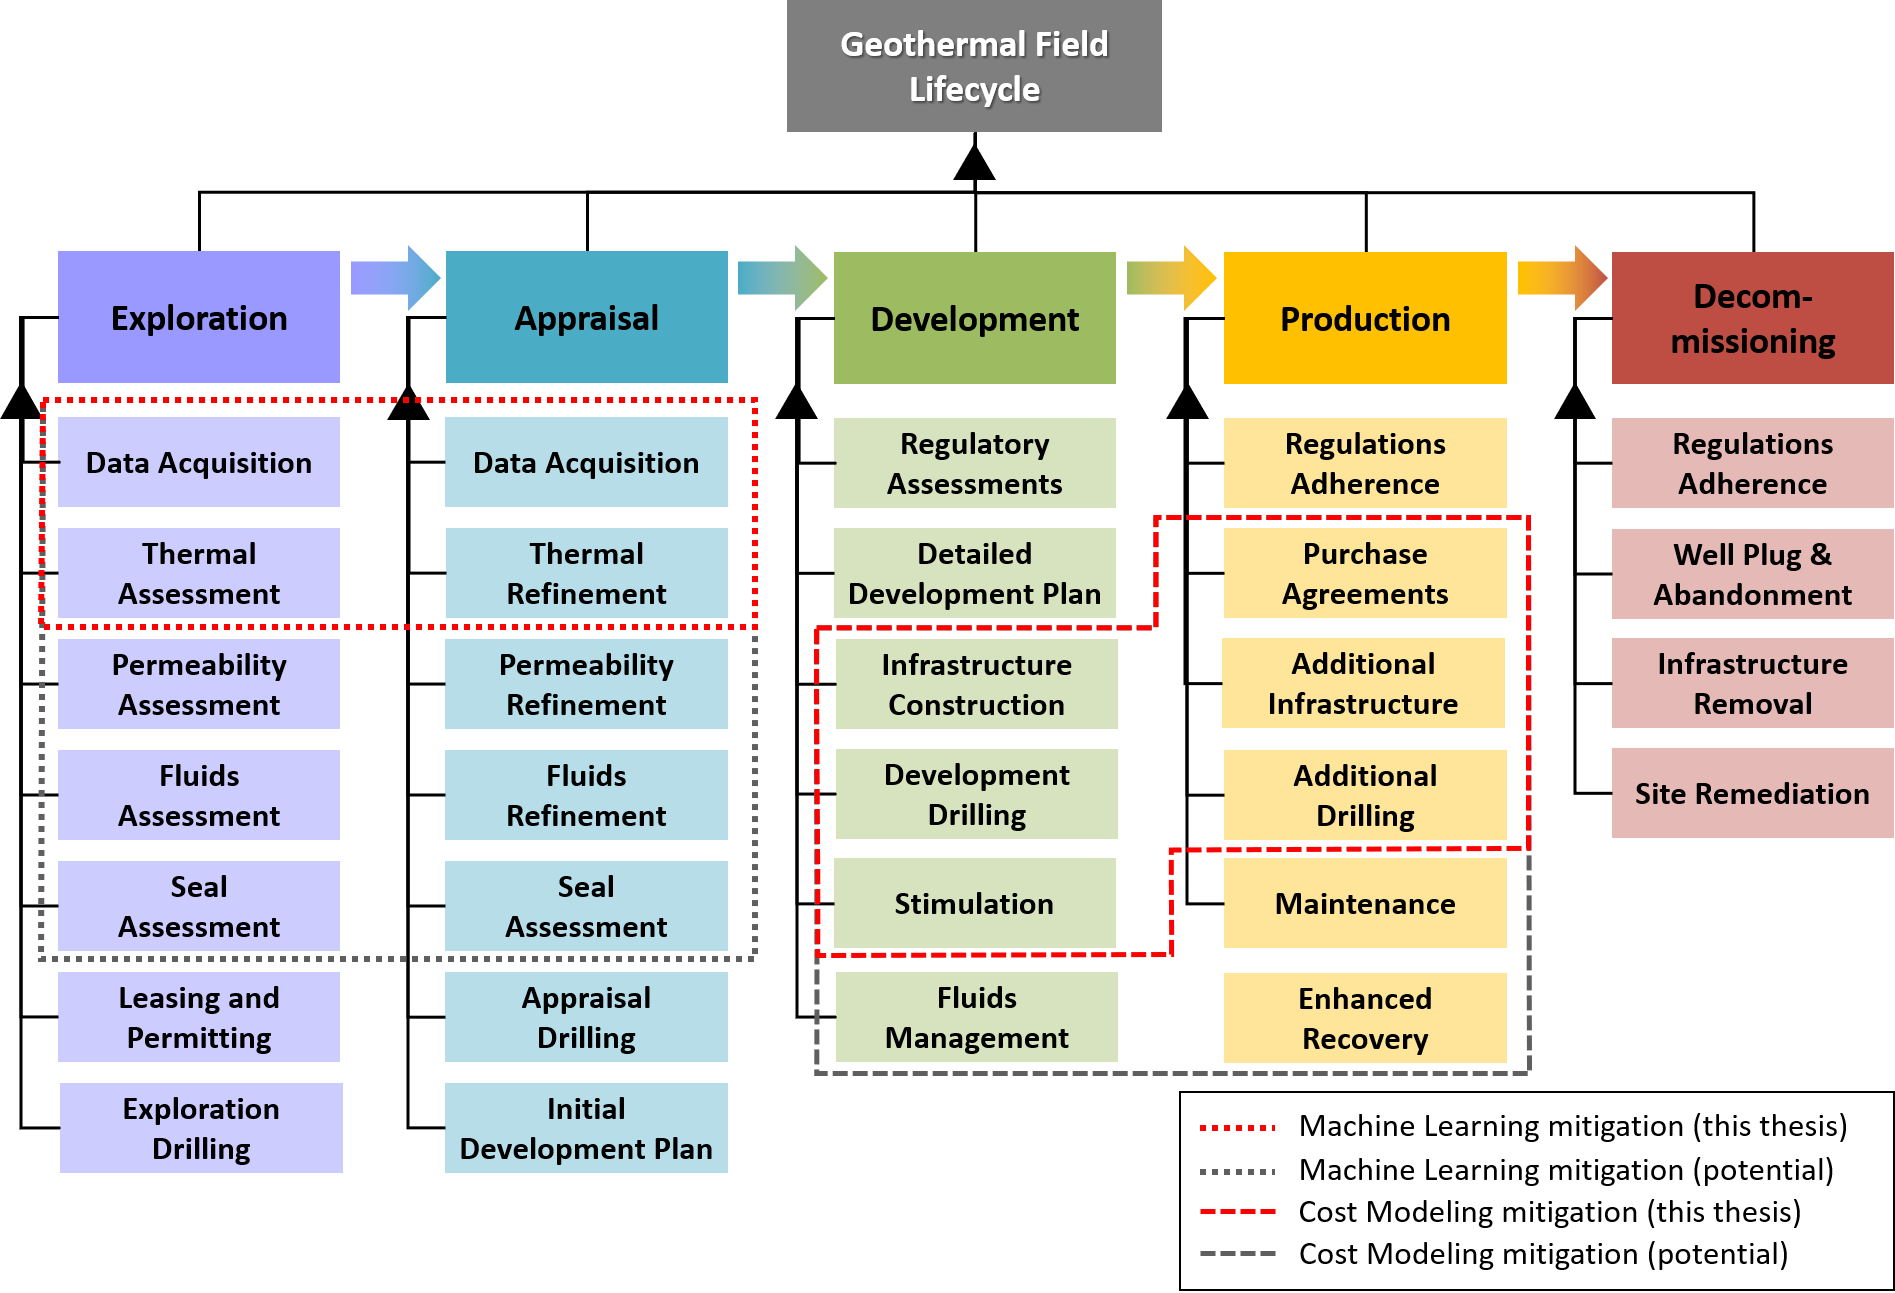
\includegraphics[width=\textwidth]{templates/images/Figure-SystemDecomposition.png}
\caption[Geothermal field lifecycle]{Proposed geothermal field lifecycle and two levels of decomposition defining major project phases and a high-level WBS. Dotted lines indicate where machine learning methods could mitigate risk in exploration and appraisal. Dashed lines depict where cost models might mitigate risk during the development and production phases.}
\label{fig:geothermal_field_lifecycle}
\end{figure}

The red dotted outline in Figure \ref{fig:geothermal_field_lifecycle} illustrates activities in the Exploration and Appraisal stages where machine learning methods described in Chapters \ref{ch3:expl_prep} and \ref{ch5:expl_ml} can reduce the overall risk profile. Geothermal exploration commonly focuses on areas where data and known resources are already present. Reviewing available data to identify feature relationships suggestive of favorable locations is an early pre-screening activity for mitigating the risk of costly exploration failures \citep{doughty_geovision_2018}. Machine learning algorithms described in Chapter \ref{ch5:expl_ml} provide data-driven methods for uncovering these complex feature relationships and generating resource favorability maps rapidly and at low cost. Furthermore, feature importances derived from recursive feature elimination (Section \ref{ch5:logreg_rfe}), impurity measures like Gini index or entropy (Section \ref{ch5:impurity}), or Shapley analysis (Section \ref{ch5:xgb_shapley}) directly rank different data sources by their value for predictive modeling. These measures could also be used to guide exploration and appraisal spending on additional data purchases or acquisition efforts. For example, recognizing that silica geothermometer temperatures, heat flow measurements, crustal thickness, and density of volcanic dikes and springs all highly influence the geothermal gradient classification model (see Section \ref{ch5:xgb_shapley}), an exploration team could focus time and budget on 1) field surveys for silica concentration sampling, 2) field or remote-sensing mapping of springs and dikes, and 3) seismic acquisition for improved crustal thickness estimates where those estimates are least well-constrained. As suggested by the black dotted line, the learnings from assessing geothermal heat content with machine learning techniques in Chapter \ref{ch5:expl_ml} are easily transferable to assessments for the other risk elements. 

Cost modeling similarly offers benefits for risk mitigation in the geothermal project lifecycle, as illustrated with the dashed lines in Figure \ref{fig:geothermal_field_lifecycle}. Surface plant construction and drilling activities take place during the development phase and continue into production as thermal decline or market forces trigger field management responses. Rather than treat the extent of these activities as known unknowns, characterizing and including them in flexible economic models offers the opportunity to assess their impact and scenario-test for the optimal field strategy. As the analysis in Chapter \ref{ch6:cm_results} showed, models can include local uncertainties, e.g., geothermal gradient or decline rate, as well as broader risks like a carbon tax or national electrification. The red long-dashed line in Figure \ref{fig:geothermal_field_lifecycle} surrounds factors considered by the cost model in Chapters \ref{ch4:cm_prep} and \ref{ch6:cm_results}. The gray dashed line depicts additional aspects of the development and production phases that could also be characterized in a cost model with distributions and decision rules to determine project viability or refine field strategy.

\section{Role of Uncertainty}
\label{ch7:uncertainty_role}

Uncertainty exists, as does the opportunity to include it in a larger decision-making process for geothermal adoption. In the exploration phase, feature standard errors and maps of entropy --- or another measure of collective uncertainty --- can influence project choices. Observing pervasively high standard errors for a data layer (see Section \ref{ch5:measure_uncertainty}) raises the question of whether that data should be re-acquired using different tools or survey methods, or if better quality data might be available for use or purchase. And zones of high entropy in measurement uncertainty highlight areas that need additional attention. Is the entropy a result of insufficient data to train machine learning models, leading to poor discrimination ability for the predicted classes? Or are the data in areas of high entropy simply inconclusive or poorly conditioned? Pursuing these questions helps frame a refined project plan for the early phases of the field lifecycle. In this scenario, time and resource allocations to data science and data engineering (using existing data), field studies and data acquisition (supplementing existing data), or exploration of more certain areas are expressly driven by the data.

If an ensemble of models is considered, structural or model uncertainty (see Section \ref{ch5:model_uncertainty}) can direct efforts around how to approach machine learning prediction. For example, when entropy appears high throughout the area of interest (AOI), and most of the models show reasonable agreement except for one or two, this could justify down-selecting those models and re-evaluating from the reduced ensemble. But if high variance is observed across many models, this might indicate the input data insufficiently describes the system. Likewise, predictions from probabilistic models that show high parameter uncertainty in the AOI (Section \ref{ch5:param_uncertainty}) should be treated as suspect and the model refactored or retrained on a larger data set. Insights like these mitigate the risk of over-confidence in under-performing models, potentially avoiding a poorly-placed exploration well based on those models further down the line.

For cost models, directly incorporating uncertainty serves to counter the classic misconception that applying average values to elements of a complex system will lead to an average system result \citep[Flaw of Averages,][p.\ 17-19]{de_neufville_flexibility_2011}. Instead, using variable distributions and generating expected values from multiple model realizations provides accurate median estimates and describes the spread of potential results. As discussed in Section \ref{ch6:cost_model_metrics}, target curves and percentiles defining Value at Risk and Value at Gain offer a richer set of metrics for model comparison. Using these metrics can reveal the combination of strategic choices for a geothermal project timeline and execution that mitigate the risk of project losses and captures the most potential gain.

\section{Risk Analysis}
\label{ch7:risk_analysis}

One approach to project risk assessment evaluates risks and mitigation actions with a scorecard tracking likelihood (Table \ref{tab:likelihood_table}) and consequence (Table \ref{tab:consequence_table}) of individual risks before and after actions are taken \citep{malone_development_2004}. The process begins with creating a risk log as shown in Table \ref{tab:risk_log}. This table can be constructed through a variety of risk identification methods, including formal hazard analysis, models and simulations, or group brainstorming \citep{nasa_s3001_2017}. Even the act of populating this table adds value to a project by building alignment on group judgment and assumptions regarding risk relevance and potential impact.

\begin{table}%[!htp]
\centering
\begin{tabular}{|c|l|c|}
\hline
\multicolumn{3}{|c|}{\textbf{Likelihood}} \\ \hline
\textbf{Score} & \multicolumn{2}{c|}{\textbf{Likelihood of Occurrence (p)}} \\ \hline
5 & Near certainty & (\ 0.8,1.0\ {]} \\ \hline
4 & Highly likely & (\ 0.6,0.8\ {]} \\ \hline
3 & Likely & (\ 0.4,0.6\ {]} \\ \hline
2 & Low likelihood & (\ 0.2,0.4\ {]} \\ \hline
1 & Not likely & {[}\ 0.0,0.2\ {]} \\ \hline
\end{tabular}
\caption[Risk likelihood]{Likelihood score based on probability of occurrence (p). Adapted from NASA S3001 Guidelines for Risk Management, v.G \protect\citep{malone_development_2004}.}
\label{tab:likelihood_table}
\end{table}

\begin{table}%[!htp]
\resizebox{\textwidth}{!}{
    \begin{tabular}{|l|L{0.17\linewidth}|L{0.17\linewidth}|L{0.17\linewidth}|L{0.17\linewidth}|L{0.17\linewidth}|}
    \hline
     & \multicolumn{5}{c|}{\textbf{Consequence}} \\ \hline
     & 1 & 2 & 3 & 4 & 5 \\ \hline
    \textbf{Performance} & Minimal to no impact on meeting project goals. & Minor impact on meeting project goals. & Unable to meet a specific project goal, but remaining goals can be achieved. & Unable to meet multiple project goals, but minimum project success still achievable. & Unable to meet multiple project goals, minimum project success not achievable. \\ \hline
    \textbf{Schedule} & Minimal to no impact on project schedule. & No change to critical milestones; at least 10-day buffer between any delay and impact on milestone timing. & No change to critical milestones; less than 10-day buffer between any delay and impact on milestone timing. & One or more critical milestones slip, impacting overall project schedule. & One or more critical milestones slip; one or more milestones cannot be achieved. \\ \hline
    \textbf{Cost} & Minimal to no impact on cost. & Minor impact on cost. Variance $< 5\%$ of total approved budget. & Impact on cost. Variance $> 5\%$ but $\leq 10\%$ of total approved budget. & Impact on cost. Variance $> 10\%$ but $\leq 15\%$ of total approved budget. & Major impact on cost. Variance $> 15\%$ of total approved budget. \\ \hline
    \end{tabular}
}
\caption[Risk consequence]{Consequence score defining the scale of impact a risk might have if it becomes a reality. Adapted from NASA S3001 Guidelines for Risk Management, v.G \protect\citep{malone_development_2004}.}
\label{tab:consequence_table}
\end{table}

\begin{table}%[!htp]
\resizebox{\textwidth}{!}{
    \begin{tabular}{|l|l|c|c|c|}
    \hline
    \multicolumn{1}{|c|}{\textbf{ID}} & \multicolumn{1}{c|}{\textbf{Description}} & \textbf{Likelihood} & \textbf{Consequence} & \textbf{Risk} \\ \hline
    EXP1 & Insufficient exploration budget & 4 & 3 & 12 \\ \hline
    EXP2 & Poor subsurface characterization & 4 & 4 & 16 \\ \hline
    EXP3 & Permitting delays & 3 & 3 & 9 \\ \hline
    DRL1 & Rig unavailability & 4 & 3 & 12 \\ \hline
    DRL2 & Drilling cost overruns & 3 & 3 & 9 \\ \hline
    DRL4 & Downhole equipment failure & 3 & 2 & 6 \\ \hline
    PRD1 & Insufficient production budget & 3 & 4 & 12 \\ \hline
    PRD4 & Rapid thermal decline & 3 & 4 & 12 \\ \hline
    PRD5 & Demand variability & 2 & 4 & 8 \\ \hline
    PRD6 & Wrong-sized infrastructure & 3 & 4 & 12 \\ \hline
    \end{tabular}
}
\caption[Geothermal risk log]{List of geothermal project risks, each assigned a likelihood of occurrence (see Table \ref{tab:likelihood_table}) and consequence (see Table \ref{tab:consequence_table}). Risk is likelihood $\times$ consequence. This list is non-exhaustive and intended to support discussion of risk matrix use.}
\label{tab:risk_log}
\end{table}

Having captured risks and ordered them by their risk score, the project team next defines mitigation plans for addressing those risks (e.g., Table \ref{tab:mitigation_log}). The resulting \textit{mitigated} risks are analyzed and assigned updated scores for likelihood and consequence, which also define the remaining risk value. Different mitigation options for the same risk can be directly compared by the final risk scores or individual likelihood or consequence scores if addressing one over the other is preferred.

\begin{table}[!htp]
\renewcommand{\arraystretch}{2.5}
\resizebox{\textwidth}{!}{
    \begin{tabular}{|l|M{0.12\linewidth}|M{0.12\linewidth}|M{0.12\linewidth}|M{0.12\linewidth}|L{0.42\linewidth}|}
    \hline
    \multicolumn{1}{|c|}{ID} & Mitigated Likelihood & Mitigated Consequence & Mitigated Risk & Risk Reduction & Mitigation Action \\ \hline
    \rowcolor[HTML]{E7E6E6} 
    EXP1 & 1 & 2 & 2 & 10 & Use ML model predictions to reduce costs in exploration \\ \hline
    \rowcolor[HTML]{E7E6E6} 
    EXP2 & 1 & 3 & 3 & 13 & Use ML for baseline model, acquire data based on importances \\ \hline
    EXP3 & 2 & 3 & 6 & 3 & Engage with regulators early to fast-track permitting \\ \hline
    DRL1 & 3 & 3 & 9 & 3 & Secure rig early and pre-plan for future drilling needs \\ \hline
    \rowcolor[HTML]{E7E6E6} 
    DRL2 & 1 & 3 & 3 & 6 & Use ML to identify high gradient areas faster, shallower drilling \\ \hline
    DRL4 & 2 & 2 & 4 & 2 & Use service companies with high-Temp equipment track record \\ \hline
    \rowcolor[HTML]{E7E6E6} 
    PRD1 & 1 & 3 & 3 & 9 & Cost modeling for optimized spending and return \\ \hline
    PRD4 & 3 & 2 & 6 & 6 & Regularly re-drill wells or re-stimulate reservoir \\ \hline
    \rowcolor[HTML]{E7E6E6}
    PRD5 & 2 & 2 & 4 & 4 & Flexibility in power generation based on market \\ \hline
    \rowcolor[HTML]{E7E6E6}
    PRD6 & 1 & 2 & 2 & 10 & Flexible design for demand-triggered capacity changes \\ \hline
    \end{tabular}}
\caption[Geothermal mitigation log]{Proposed mitigations for risks listed in Table \ref{tab:risk_log} and the change in risk associated with those mitigations. Risk values are likelihood $\times$ consequence. Shaded mitigations include one of the options described in this thesis and appear in Figure \ref{fig:risk_matrix}. Adapted from NASA S3001 Guidelines for Risk Management, v.G (Malone \& Moses, 2004). }
\label{tab:mitigation_log}
\end{table}

The risk scorecard methodology plots risks before and after mitigation on a $5\times5$ matrix, where high-likelihood, high-consequence risks fall near the upper-right, and the lower-left represents the ideal low-likelihood, minimal-consequence region. The risk matrix serves two main functions: prioritization and selection. First, it quickly differentiates between risks by using assigned risk priorities for each matrix cell. Following NASA guidelines, priority values across the matrix increase toward the upper-right, are non-symmetric, and skew higher for high-consequence cells \citep{nasa_s3001_2017}. Secondly, different mitigation strategies for the same risk can be evaluated and plotted in the same $5\times5$. This helps quickly communicate relative outcomes of different strategies and supports rapid decision-making on which to select.

\begin{figure}%[htp]
\centering
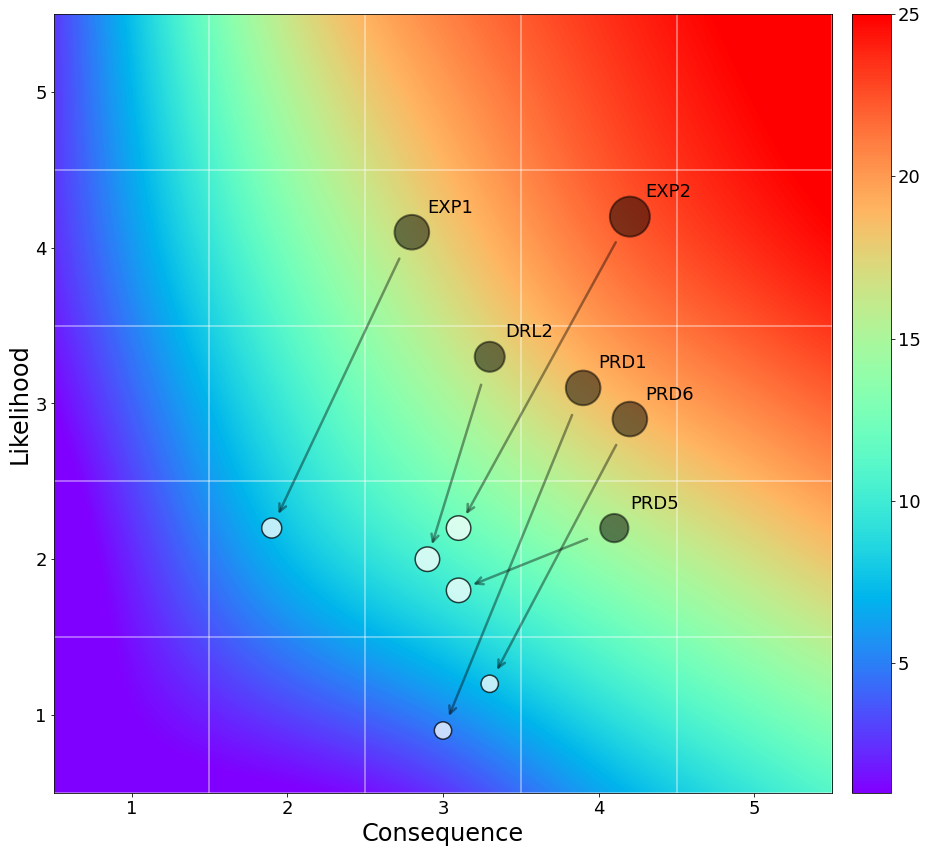
\includegraphics[width=\linewidth]{templates/images/Figure-Risk_Matrix.png}
\caption[Geothermal project risk matrix]{Risk matrix for categorizing and prioritizing project risks (dark gray) and charting risk mitigation strategies (white). Marker size corresponds with risk value (likelihood $\times$ consequence). Markers are spread out within each cell for visualization purposes. Risk labels match those in Table \ref{tab:risk_log}.}
\label{fig:risk_matrix}
\end{figure}

Figure \ref{fig:risk_matrix} illustrates a risk matrix based on the highlighted rows from Table \ref{tab:mitigation_log}. Arrows map the original risk to mitigated risk. Each of these examples utilizes mitigation strategies described in the earlier chapters of this thesis. Although many other geothermal project risks exist than those described here, what this work demonstrates is the ability \textit{to} reduce risk \textit{by} rapidly applying low-cost assessments throughout the lifecycle of a geothermal field \textit{using} readily-available data. At the exploration stage, machine-learning PFA assessments feed directly into risking processes already common in oil \& gas companies \citep{nash_adaptation_2015}. This reduces barriers around deployment and adoption, and the risk reduction in Figure \ref{fig:risk_matrix} clearly demonstrates the potential value gained. In the development and production stages, use of scenario-testing with flexible cost models mitigates risk while possibly revealing new, more profitable means of operating a geothermal field. And doing so with spreadsheet-based tools means petroleum industry project managers already have the technology and capability to apply these models for decision-support and risk-mitigation today. 

\section{Great Opportunity}

Oil \& gas companies are uniquely positioned to embrace geothermal, including EGS, as a low-carbon baseload option in the energy transition. Consider some present-day barriers to broad commercial development of EGS described in the GeoVision study: 
\begin{enumerate}
    \item \textit{Companies advancing EGS are small, lacking significant operating capital and the ability to tackle large-scale projects (>100 MW)} \citep{doughty_geovision_2018}. Oil \& gas companies have the working capital to take on larger, more expensive projects if those projects have the potential for long-term profitability.
    \item \textit{Subsurface characterization with advanced methods like seismic imaging and reservoir modeling require capabilities not generally found in the geothermal industry} \citep{doughty_geovision_2018}. Use of the most advanced geophysical data processing techniques, cutting-edge interpretation platforms, and 3D earth modeling methods are standard practice in the petroleum industry.
    \item \textit{Geothermal practitioners lack standardization or best practices for drilling complex wells} \citep{doughty_geovision_2018}. Oil \& gas companies follow standard procedures in drilling operations founded on years of experience drilling wells all across the globe, including in environments challenged by extreme depths, complex geology, and high temperatures and pressures.
    \item \textit{EGS requires complex subsurface operations like directional drilling and multi-zonal isolation for fracture stimulation not typical of traditional hydrothermal operations} \citep{augustine_geovision_2019}. Technology improvements and years of expertise gained from developing unconventional reservoirs have created a wealth of experience in directional drilling and fracking within the oil \& gas industry.
\end{enumerate}

Interest in collaboration runs high as well. The Geothermal Technologies Office regularly promotes cross-over technology transfer between the oil \& gas and geothermal communities, funding programs like GEO out of the University of Texas Austin that specifically target transitioning industry capabilities \citep{hamm_geothermal_2021}. And the operational efficiencies that companies like Unocal previously brought to geothermal operations in the United States, Philippines, and Indonesia in the past resonate with the needs of today \citep{melosh_geothermal_2017,palma_dynamic_2014}.

Given the promise of change in the energy transition, the cross-sector synergies in fundamental skill sets, and strong interest in partnership from those already committed, geothermal may be the shortest path solution for building a lower-carbon business portfolio. Getting there requires analysis of the risks as well as mitigation strategies needed to reduce the likelihood and consequence of those risks, as described in Section \ref{ch7:risk_analysis}. Based on the results of this thesis, the path from great opportunity to profitability may lie in combining available data and digital technologies to create useful predictive models with uncertainty. The last part is fundamental --- uncertainty analysis will define where measurements are meaningful, where models are predictive, and which strategy offers the greatest potential gain. Lessons learned here apply to geothermal exploration and production, but embracing uncertainty for better decision-making and risk-mitigation will likely benefit every stage of the geothermal lifecycle. Uncertainty characterization may thus be the key to building more certainty in the future of geothermal.